\begin{homeworkProblem}[2]
For each sub-problem, subfigure (a) displays the cobwebbing method result, with an initial value slight off (add perturbation) the steady state,
and guess from the plot whether the steady state is stable or not. To be more
confident, the conclusions will be tested by calculation.

\begin{enumerate}
% Problem 2(a)
\item The steady state $\bar x$ for equation $x_{n+1} = rx_n(1-x_n)$ is
$\bar x = 0$. Since there's one arbitrary constant $r$, whether the steady
state is stable or not depends on the value of $r$.

We first try $r=2$:
\begin{figure}[h]
    \centering
    \begin{subfigure}[t]{0.4\linewidth}
        \centering
        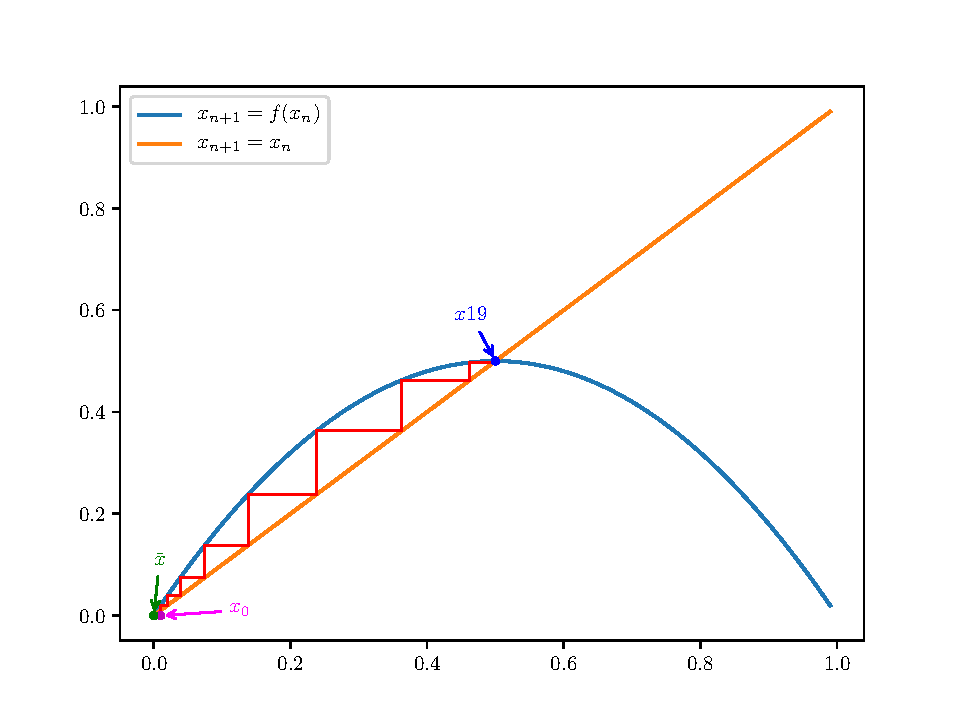
\includegraphics[scale=0.5]{fig/fig2(a)(1)_cob.pdf}
        \caption{$x_{n+1}\ v.s.\ x_n$}
    \end{subfigure}
    \hfill
    \begin{subfigure}[t]{0.4\linewidth}
        \centering
        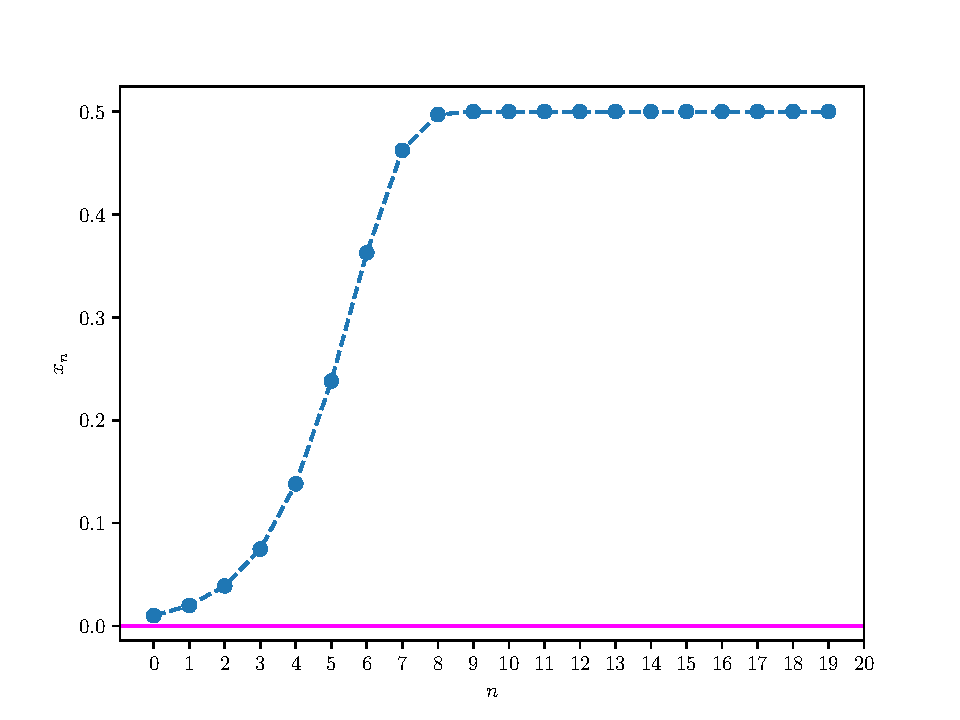
\includegraphics[scale=0.5]{../fig/fig2(a)(1).pdf}
        \caption{$x_{n+1}\ v.s.\ n$}
    \end{subfigure}
    \caption[The behavior of equation $x_{n+1} = 2x_n(1-x_n)$]{
    The behavior of equation $x_{n+1} = 2x_n(1-x_n)$,
    The steady state is marked by the horizontal magenta line.}
    \label{fig:fig2a1}
\end{figure}

It's clear in Figure \ref{fig:fig2a1} that when $r=2$, $\bar x = 0$ is not a
stable steady state.

The next try is $r=0.5$:
\begin{figure}[h]
    \centering
    \begin{subfigure}[t]{0.4\linewidth}
        \centering
        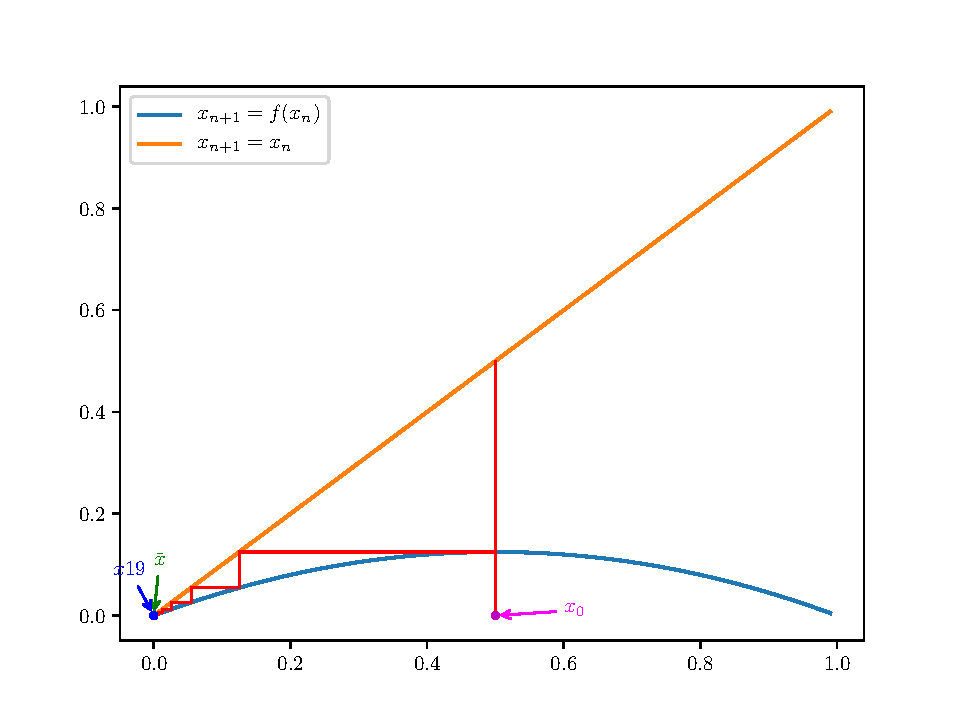
\includegraphics[scale=0.5]{fig/fig2(a)(2)_cob.pdf}
        \caption{$x_{n+1}\ v.s.\ x_n$}
    \end{subfigure}
    \hfill
    \begin{subfigure}[t]{0.4\linewidth}
        \centering
        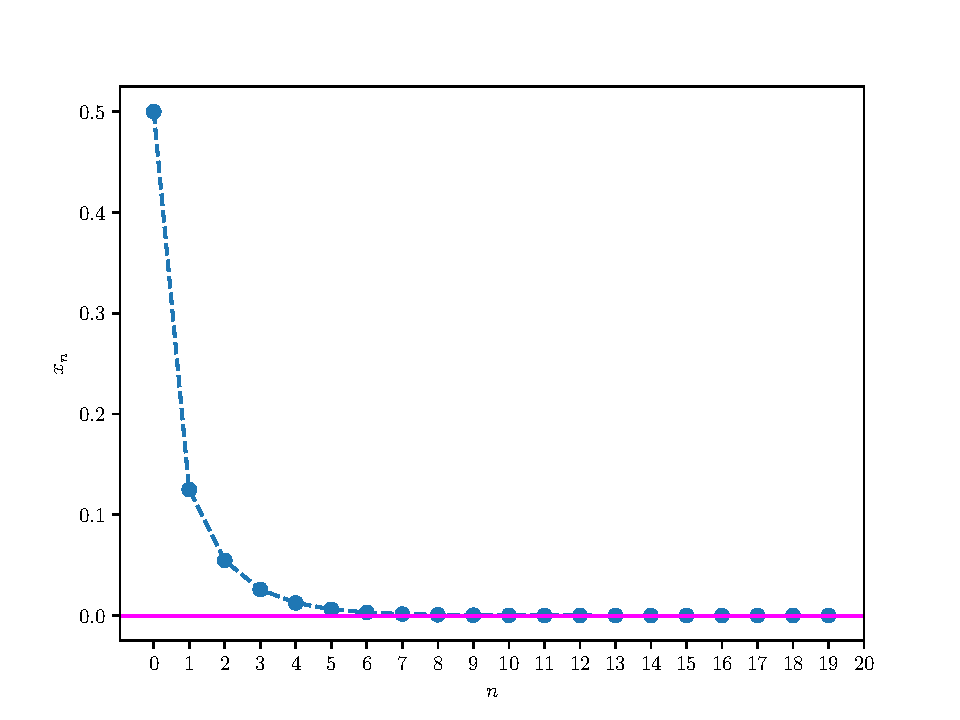
\includegraphics[scale=0.5]{../fig/fig2(a)(2).pdf}
        \caption{$x_{n+1}\ v.s.\ n$}
    \end{subfigure}
    \centering
    \caption[The behavior of equation $x_{n+1} = \frac{x_n(1-x_n)}{2}$]{
    The behavior of equation $x_{n+1} = \frac{x_n(1-x_n)}{2}$,
    The steady state is marked by the horizontal magenta line.}
    \label{fig:fig2a2}
\end{figure}
It seems that when $r = 0.5$, $\bar x = 0$ is a stable steady state. It's
intuitive to guess that probably $r < 1$ will make $\bar x = 0$ be stable.

Further exploration is shown in Figure \ref{fig:fig2a3} below:
\begin{SCfigure}[1][h]
    \centering
    \caption[The behavior of equations $x_{n+1} = rx_n(1-x_n)$]{
    The behavior of equations $x_{n+1} = rx_n(1-x_n)$, with $r \in \{
        -1, -0.95, -0.5, 0.5, 0.7,0.8, 0.9, 0.95, 0.98, 1
    \}$. It can be seen that the all equations except for the one with $r = -1$
    converges to the steady state (marked by the magenta horizontal line).}
    \label{fig:fig2a3}
    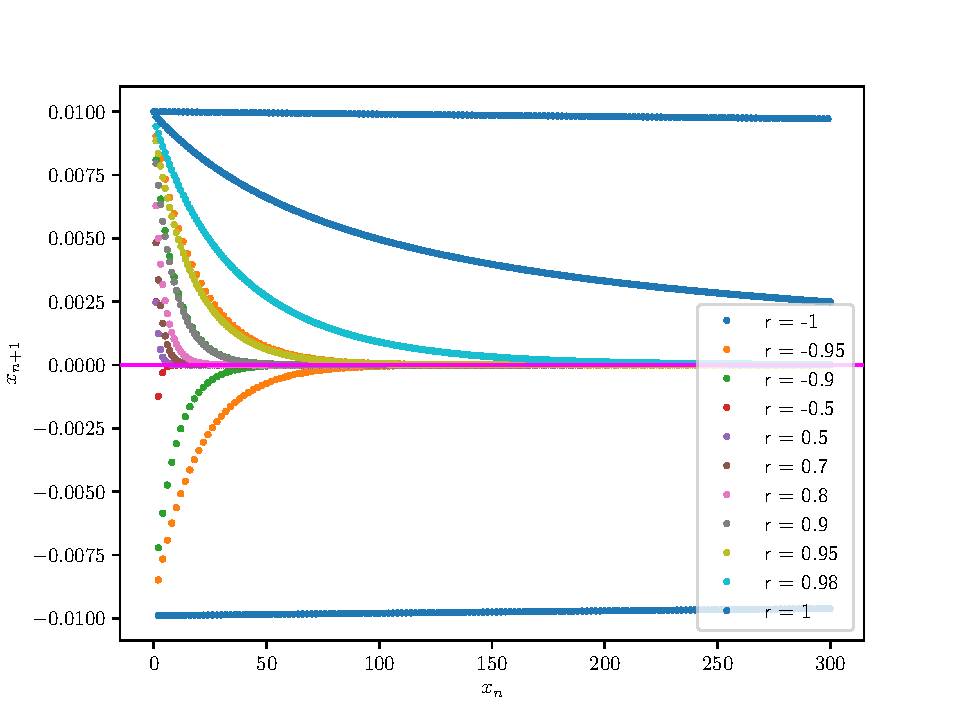
\includegraphics[scale=0.6]{../fig/fig2(a)(3).pdf}
\end{SCfigure}

It seems that for $-1 < r < 1$, or $|r| < 1$, $\bar x = 0$ will be a stable
steady state. That is to say, even with small perturbation (here is $x' = 0.01$)
present, the equation still can eventually reach the steady state.

\segline

\subsection{Test}
Recall \[
    \boxed{
    \bar x \text{ is a stable steady state}
    \Longleftrightarrow
    \left| \left.\deriv{f}\right|_{\bar x} \right| < 1
    }
\]
We can derive that
\[
    \begin{aligned}
        &\left|\left.\derivlong{rx(1-x)}\right|_{\bar x}\right|\\
        &\qquad = \left| \left.(r - 2rx)\right|_{\bar x} \right|\\
        &\qquad = |r| < 1
    \end{aligned}
\]
It confirms with our conclusion that when $|r| < 1$, $\bar x = 0$ will be a
stable steady state.
\pagebreak
\item Plotting the figure of equation $x_{n+1} = -x_n^2(1-x_n)$ with initial
condition $x_0 = 1.6$ slightly off the given steady state $\bar x = (1+ \sqrt{5}
)/2$ gives:
\begin{figure}[h]
    \centering
    \begin{subfigure}[t]{0.4\linewidth}
        \centering
        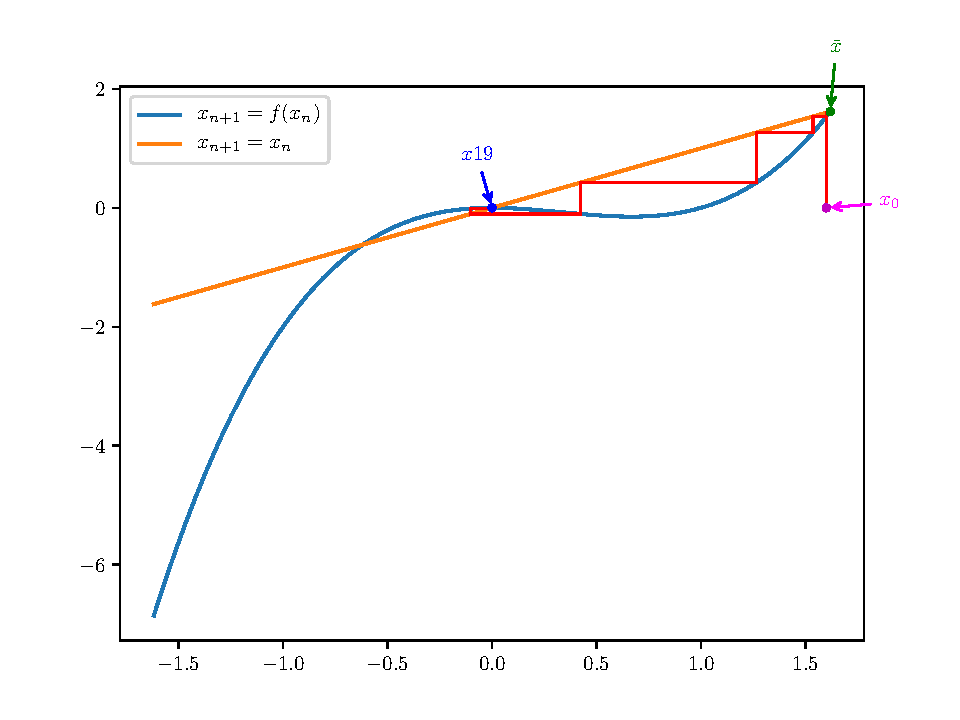
\includegraphics[scale=0.5]{fig/fig2(b)_cob.pdf}
        \caption{$x_{n+1}\ v.s.\ x_n$}
    \end{subfigure}
    \hfill
    \begin{subfigure}[t]{0.4\linewidth}
        \centering
        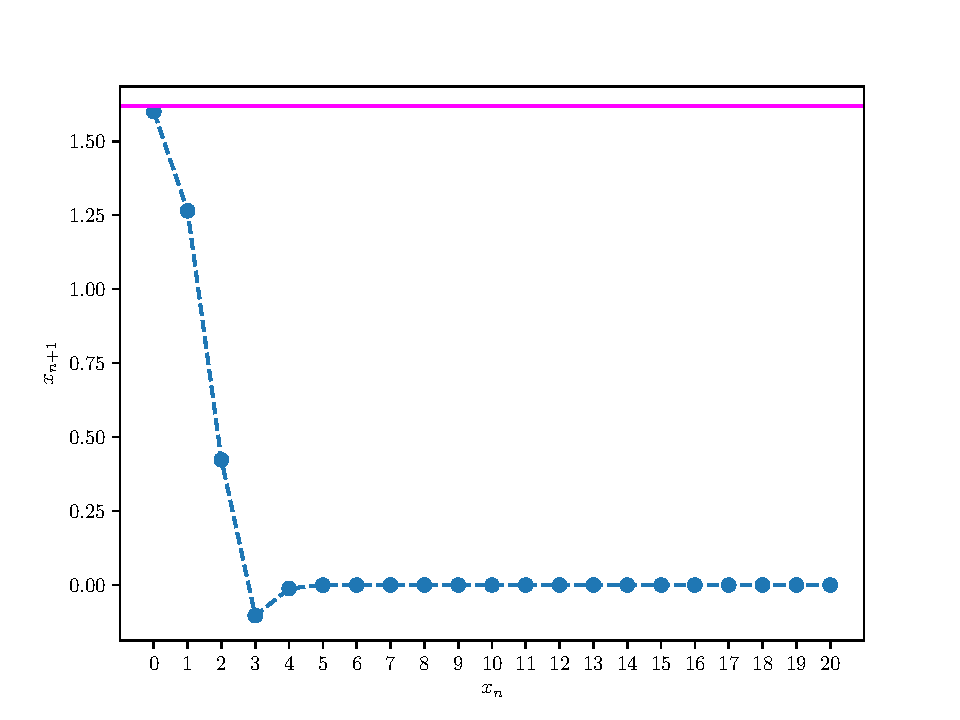
\includegraphics[scale=0.5]{../fig/fig2(b).pdf}
        \caption{$x_{n+1}\ v.s.\ n$}
    \end{subfigure}
    \centering
    \caption{The behavior of equation $x_{n+1} = -x_n^2(1-x_n)$}
\end{figure}
\\
We can see that the steady state is unstable. The calculation of condition:
\[
    \begin{aligned}
        &\left|\left.\derivlong{-x^2(1-x)}\right|_{\bar x}\right|\\
        &\qquad = \left| \left.(-2x + 3x^2)\right|_{\bar x} \right|\\
        &\qquad = \frac{7+\sqrt{5}}{2} > 1
    \end{aligned}
\]
also confirms that $\bar x = (1+\sqrt{5})/2$ is not stable.

\item Plotting the figure of equation $x_{n+1} = 1/(2+x_n)$ with initial
condition $x_0 = 0.4$ slightly off the given steady state $\bar x = \sqrt{2}
- 1$ gives:
\begin{figure}[h]
    \centering
    \begin{subfigure}[t]{0.4\linewidth}
        \centering
        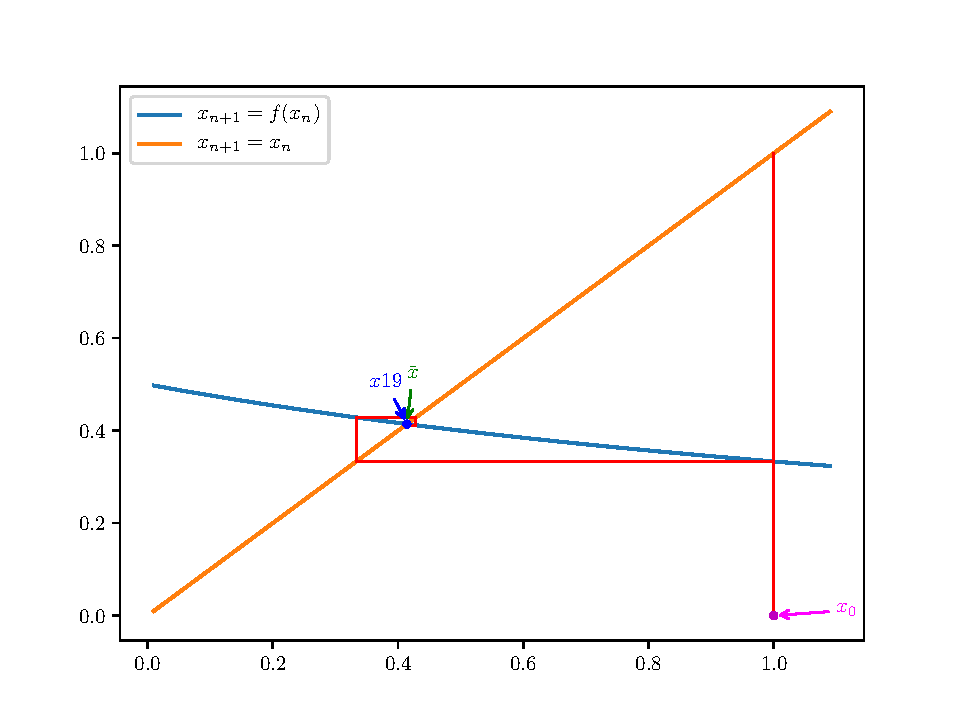
\includegraphics[scale=0.5]{fig/fig2(c)_cob.pdf}
        \caption{$x_{n+1}\ v.s.\ x_n$}
    \end{subfigure}
    \hfill
    \begin{subfigure}[t]{0.4\linewidth}
        \centering
        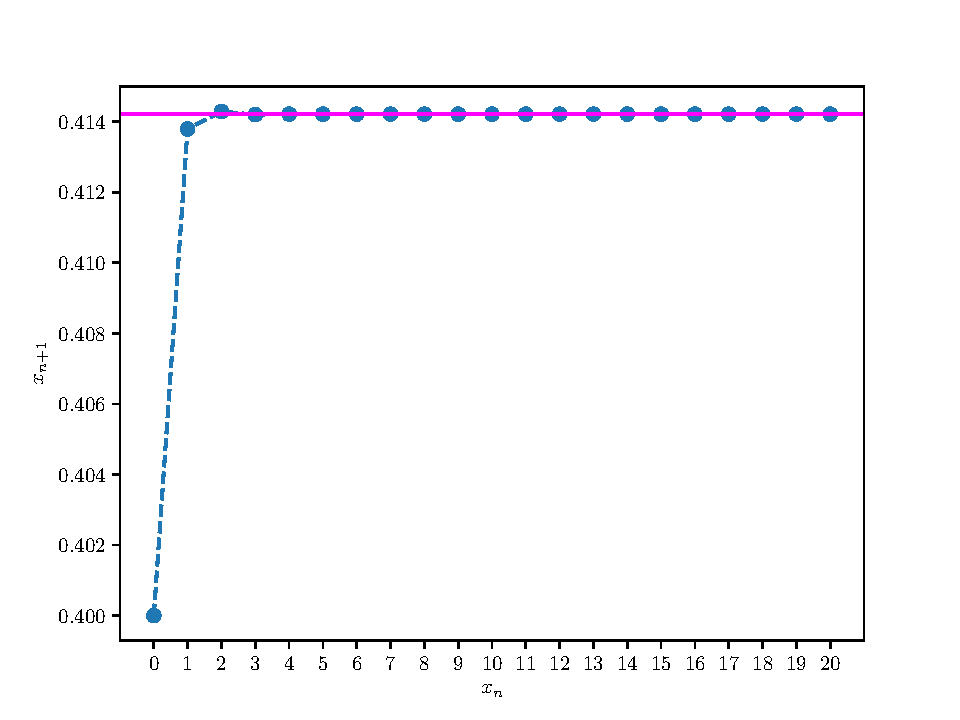
\includegraphics[scale=0.5]{../fig/fig2(c).pdf}
        \caption{$x_{n+1}\ v.s.\ n$}
    \end{subfigure}
    \centering
    \caption{The behavior of equation $x_{n+1} = 1/(2+x_n)$}
\end{figure}
\\
We can see that the steady state is stable. The calculation of condition:
\[
    \begin{aligned}
        &\left|\left.\derivlong{1/(2+x)}\right|_{\bar x}\right|\\
        &\qquad = \left| \left.\left(\frac{-1}{(2+x)^2}\right)\right|_{\bar x}
        \right|\\
        &\qquad = 3 - 2\sqrt{2} < 1
    \end{aligned}
\]
also confirms that $\bar x = \sqrt{2} - 1$ is stable.

\item Plotting the figure of equation $x_{n+1} = x_n \ln x_n^2$ with initial
condition $x_0 = 1.648$ slightly off the given steady state $\bar x = e^{1/2}$
gives:
\begin{figure}[h]
    \centering
    \begin{subfigure}[t]{0.4\linewidth}
        \centering
        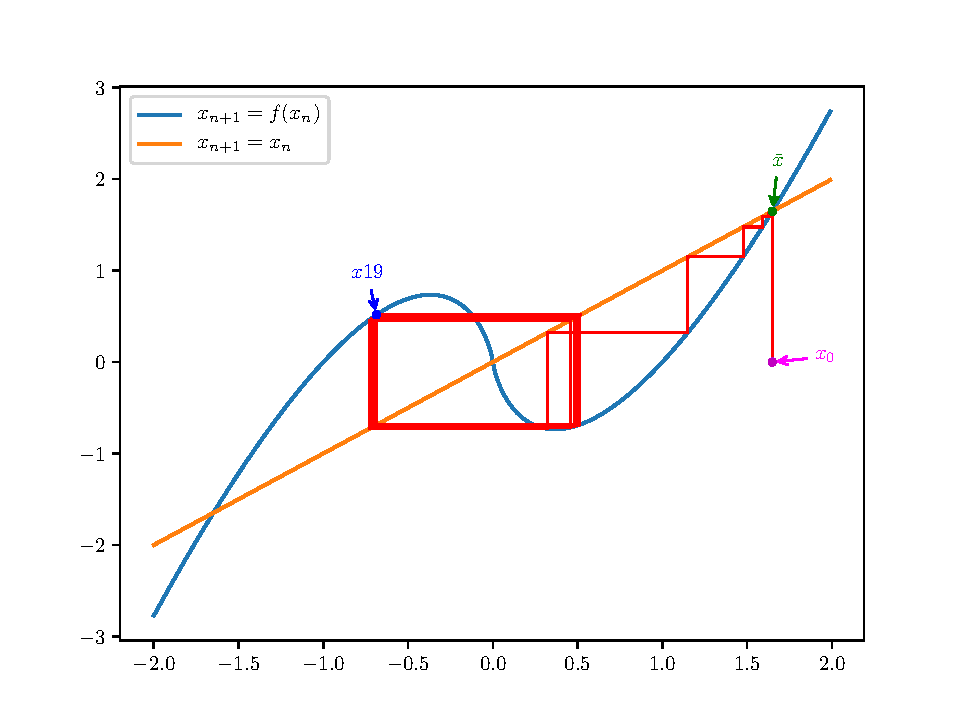
\includegraphics[scale=0.5]{fig/fig2(d)_cob.pdf}
        \caption{$x_{n+1}\ v.s.\ x_n$}
    \end{subfigure}
    \hfill
    \begin{subfigure}[t]{0.4\linewidth}
        \centering
        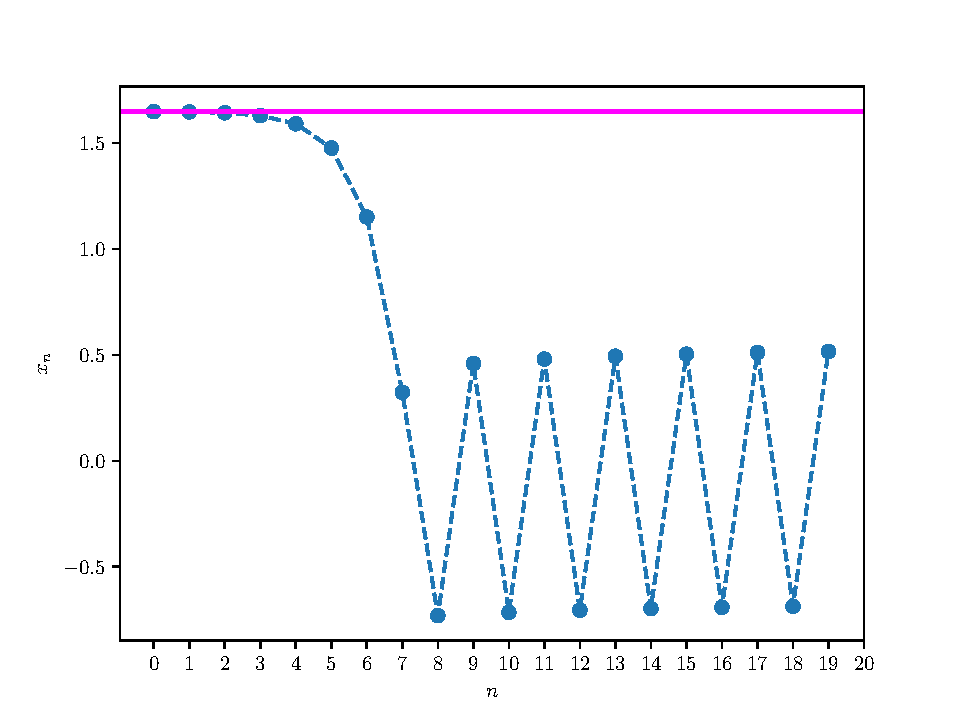
\includegraphics[scale=0.5]{../fig/fig2(d).pdf}
        \caption{$x_{n+1}\ v.s.\ n$}
    \end{subfigure}
    \centering
    \caption{The behavior of equation $x_{n+1} = x_n \ln x_n^2$}
\end{figure}
\\
We can see that the steady state is unstable. The calculation of condition:
\[
    \begin{aligned}
        &\left|\left.\derivlong{x\ln x^2}\right|_{\bar x}\right|\\
        &\qquad = 2.5 > 1
    \end{aligned}
\]
also confirms that $\bar x = e^{1/2}$ is not stable.
\end{enumerate}
\end{homeworkProblem}